\documentclass[conference]{IEEEtran}

\usepackage{cite}
\usepackage{amsmath,amssymb,amsfonts}
\usepackage{graphicx}
\usepackage{textcomp}
\usepackage{xcolor}
\usepackage{hyperref}
\usepackage{booktabs}
\usepackage{multirow}
\usepackage{listings}
\usepackage{balance}

\lstset{
  basicstyle=\ttfamily\small,
  breaklines=true,
  frame=single,
  xleftmargin=1em,
}

\graphicspath{{../results/figures/}}

\begin{document}

\title{AutoNAT v2: Performance Analysis and Cross-Implementation Study of libp2p's Reachability Protocol}

\author{
\IEEEauthorblockN{Sergi Pont}
\IEEEauthorblockA{ProbeLab, Protocol Labs\\
sergi@probelab.io}
}

\maketitle

\begin{abstract}
AutoNAT v2 is libp2p's protocol for determining whether a node's network addresses are publicly reachable. It replaces AutoNAT v1's global majority-vote model with per-address testing, nonce-based verification, and amplification protection. We present the first systematic evaluation of AutoNAT v2 across three implementations (go-libp2p, rust-libp2p, js-libp2p) using a Docker-based testbed with configurable NAT types, network degradation, and OpenTelemetry tracing.

Across 178 controlled experiments spanning 5 NAT configurations, 2 transport protocols, and varying latency/packet-loss conditions, we find that AutoNAT v2 achieves 0\% false negative and 0\% false positive rates for standard NAT types with ${\sim}6$-second convergence. However, we identify 10 findings that affect real-world deployment: (1) v2 results are not consumed by the DHT or relay subsystems in go-libp2p---v1 still controls these, and v1 oscillates in 60\% of runs with unreliable peers; (2) rust-libp2p probes ephemeral ports instead of listen addresses, producing 100\% false negatives; (3) the protocol cannot distinguish address-restricted from full-cone NAT, producing 100\% false positives for ADF NATs; (4) under symmetric NAT, no address reaches the activation threshold, producing no signal at all. Only go-libp2p (via Kubo) deploys v2 in production. We propose recommendations for each implementation and a NAT monitoring service for real-world validation.
\end{abstract}

\begin{IEEEkeywords}
NAT traversal, libp2p, AutoNAT, peer-to-peer, reachability detection, IPFS, QUIC
\end{IEEEkeywords}

%----------------------------------------------------------------------
\section{Introduction}
%----------------------------------------------------------------------

Peer-to-peer networks require nodes to know whether they are reachable from the internet. A node behind Network Address Translation (NAT) has a private IP address that is not directly routable---other peers cannot initiate connections to it. Without reachability detection, such nodes may advertise unreachable addresses, operate as DHT servers when they should be clients, or fail to reserve relay connections they need for connectivity.

The libp2p networking stack~\cite{libp2p-specs} addresses this with AutoNAT---a protocol where a node asks peers to test whether its addresses are dialable from outside. AutoNAT v1~\cite{autonat-v1} uses a simple model: the node asks a random connected peer to dial it back, and accumulates a global Public/Private verdict from a sliding window of results. AutoNAT v2~\cite{autonat-v2-spec}, specified in 2023 and first implemented in go-libp2p v0.34.0 (May 2024), improves on this with per-address testing, nonce-based dial-back verification, and amplification attack protection.

Despite its deployment in Kubo (the primary IPFS implementation, with tens of thousands of nodes), no systematic evaluation of AutoNAT v2 exists. The protocol has three independent implementations (Go, Rust, JavaScript), but cross-implementation interoperability and correctness have not been tested.

\subsection{Contributions}

\begin{enumerate}
\item \textbf{First cross-implementation evaluation of AutoNAT v2.} We test go-libp2p, rust-libp2p, and js-libp2p implementations against go-libp2p servers in a controlled testbed with 5 NAT types.
\item \textbf{Quantitative performance characterization.} 178 experiments measuring false negative/positive rates, time-to-confidence, time-to-update, and transport-specific resilience (TCP vs QUIC).
\item \textbf{Identification of 10 findings} spanning protocol design, implementation, and integration issues---including 3 high-severity findings affecting DHT participation.
\item \textbf{Actionable recommendations} for each implementation, the protocol specification, and the broader ecosystem.
\item \textbf{A proposal for real-world validation} using DHT sybil nodes to classify NAT types across the live IPFS network.
\end{enumerate}

%----------------------------------------------------------------------
\section{Background}
%----------------------------------------------------------------------

\subsection{NAT Types}

NAT behavior is defined by two independent properties~\cite{rfc4787}: \emph{mapping} (how the router assigns external ports) and \emph{filtering} (which inbound packets pass through). Table~\ref{tab:nat-types} summarizes the four NAT configurations relevant to this study.

\begin{table}[htbp]
\caption{NAT Type Classification (RFC 4787)}
\label{tab:nat-types}
\centering
\begin{tabular}{@{}llll@{}}
\toprule
NAT Type & Mapping & Filtering & Inbound \\
\midrule
Full-cone & EIM & EIF & Always \\
Addr-restricted & EIM & ADF & Contacted IPs \\
Port-restricted & EIM & APDF & Exact IP:port \\
Symmetric & ADPM & APDF & Never \\
\bottomrule
\end{tabular}
\end{table}

Endpoint-Independent Mapping (EIM) assigns the same external port regardless of destination. Address- and Port-Dependent Mapping (ADPM) assigns a different port per destination. Filtering ranges from Endpoint-Independent (EIF, allows any source) through Address-Dependent (ADF, allows previously contacted IPs) to Address- and Port-Dependent (APDF, requires exact IP:port match).

\subsection{libp2p Protocol Stack}

AutoNAT operates within a protocol ecosystem where each component handles a different aspect of connectivity:

\textbf{Identify} (\texttt{/ipfs/id/1.0.0}): Peers exchange metadata including the \texttt{ObservedAddr}---the address each sees the other connecting from. Go-libp2p's \texttt{ObservedAddrManager} consolidates these: an address must be reported by $\geq$\texttt{ActivationThresh} (default: 4) distinct observers before promotion.

\textbf{AutoNAT v1} (\texttt{/libp2p/autonat/1.0.0}): Global reachability via random peer dial-back. Sliding window of 3 results. The Kademlia DHT subscribes to this verdict.

\textbf{AutoNAT v2} (\texttt{/libp2p/autonat/2/dial-request}): Per-address testing with nonce verification. \texttt{targetConfidence=3} in sliding window of 5. The DHT does \emph{not} subscribe to v2.

\textbf{Circuit Relay v2} and \textbf{DCUtR}: When behind NAT, a node reserves a relay slot; DCUtR attempts hole punching through the relay.

\subsection{AutoNAT v1 vs v2}

Table~\ref{tab:v1v2} compares the two protocol versions.

\begin{table}[htbp]
\caption{AutoNAT v1 vs v2 Comparison}
\label{tab:v1v2}
\centering
\begin{tabular}{@{}lll@{}}
\toprule
Aspect & v1 & v2 \\
\midrule
Scope & Global & Per-address \\
Probing & Random peer & Server selection \\
Confidence & Window of 3 & Window of 5, target=3 \\
Nonce & No & Yes \\
Amplification prot. & No & 30--100\,KB \\
Dial-back identity & Same ID & Separate ID \\
DHT consumes & \textbf{Yes} & \textbf{No} \\
\bottomrule
\end{tabular}
\end{table}

\subsection{Related Work}

Trautwein et al.~\cite{trautwein2022} measured decentralized hole punching across IPFS, finding ${\sim}70\%$ success rate. Their follow-up~\cite{trautwein2025} analyzed 4.4M+ traversal attempts, confirming the baseline and refuting the assumption of UDP superiority. Halkes and Pouwelse~\cite{halkes2011} measured NAT puncturing, finding ${\sim}82\%$ of NATs support UDP hole punching and ${\sim}11\%$ of peers are behind symmetric NAT.

RFC~4787~\cite{rfc4787} defines NAT behavioral requirements. RFC~7857~\cite{rfc7857} updates these toward protocol-dependent endpoint-independent filtering. To our knowledge, no prior work has evaluated AutoNAT v2 specifically, nor compared its behavior across implementations.

%----------------------------------------------------------------------
\section{Testbed Design}
%----------------------------------------------------------------------

\subsection{Architecture}

We designed a Docker-based testbed with configurable NAT types implemented via iptables rules. The testbed consists of two networks: a ``public'' network (73.0.0.0/24, using a public-looking range because go-libp2p's \texttt{manet.IsPublicAddr()} filters private/CGNAT ranges) and a private network (10.0.1.0/24). A router container implements all 5 NAT types via iptables masquerade and filtering rules, with \texttt{tc netem} for latency/packet-loss injection.

Servers (3--7 go-libp2p nodes) run AutoNAT v2 from our instrumented fork~\cite{probelab-fork} with OpenTelemetry tracing. Client nodes (go-libp2p, rust-libp2p, or js-libp2p) sit behind the router and export OTel spans to Jaeger. A Python orchestrator manages Docker Compose lifecycles and exports traces as JSONL.

\subsection{Instrumentation}

We added OpenTelemetry tracing to go-libp2p's AutoNAT v2 client: \texttt{autonatv2.probe} (per-probe), \texttt{autonatv2.refresh\_cycle} (confidence cycle), and \texttt{autonatv2.server\_selection}. All client implementations emit compatible application-level spans (\texttt{reachable\_addrs\_changed}, \texttt{reachability\_changed}).

\subsection{Experiments}

Table~\ref{tab:experiments} summarizes the experiment matrix.

\begin{table}[htbp]
\caption{Experiment Matrix}
\label{tab:experiments}
\centering
\begin{tabular}{@{}lrr@{}}
\toprule
Experiment & Scenarios & Runs \\
\midrule
Baseline (5 NATs $\times$ 2 transports) & 10 & 10 \\
High latency (4$\times$2$\times$\{200,500\}ms) & 16 & 16 \\
Packet loss (4$\times$2$\times$\{1,5,10\}\%) & 24 & 24 \\
ADF false positive (2$\times$3$\times$20 runs) & 6 & 120 \\
Toggle detection (5 combos $\times$ 2 phases) & 5 & 5 \\
v1/v2 gap (600s observation) & 2 & 5 \\
Threshold sensitivity & 6 & 6 \\
\midrule
\textbf{Total} & \textbf{69} & \textbf{178} \\
\bottomrule
\end{tabular}
\end{table}

%----------------------------------------------------------------------
\section{Results: Baseline Performance}
%----------------------------------------------------------------------

\subsection{Correctness}

Across all non-edge-case scenarios (full-cone, port-restricted, no-NAT), AutoNAT v2 achieves \textbf{0\% FNR} and \textbf{0\% FPR}. These results hold across all latencies (up to 500\,ms one-way) and packet loss rates (up to 10\%).

\subsection{Convergence Time}

Baseline time-to-confidence with 7 servers (Table~\ref{tab:baseline}): ${\sim}6$\,s for reachable nodes (3 probes $\times$ ${\sim}2$\,s per cycle), ${\sim}6$--11\,s for unreachable (QUIC port-restricted requires an extra round).

\begin{table}[htbp]
\caption{Baseline Time-to-Confidence (7 servers)}
\label{tab:baseline}
\centering
\begin{tabular}{@{}lrrl@{}}
\toprule
NAT Type & TCP (ms) & QUIC (ms) & Result \\
\midrule
Full-cone & 6,022 & 6,021 & Reachable \\
Addr-restricted & 6,021 & 6,021 & Reachable (FP) \\
Port-restricted & 6,013 & 11,015 & Unreachable \\
Symmetric & --- & --- & No signal \\
\bottomrule
\end{tabular}
\end{table}

\subsection{Transport Resilience}

QUIC is dramatically more resilient to packet loss than TCP (Table~\ref{tab:resilience}). At 10\% loss, TCP convergence nearly triples while QUIC is essentially unaffected. QUIC handles retransmission at the transport layer, absorbing loss before AutoNAT observes it. Correctness (0\% FNR/FPR) is unaffected in all conditions.

\begin{table}[htbp]
\caption{TTC Increase Under Network Degradation}
\label{tab:resilience}
\centering
\begin{tabular}{@{}lrr@{}}
\toprule
Condition & TCP increase & QUIC increase \\
\midrule
1\% loss & +0\% & +0\% \\
5\% loss & +17\% & +4\% \\
10\% loss & \textbf{+147\%} & \textbf{+1\%} \\
200\,ms latency & +210\% & +110\% \\
500\,ms latency & +432\% & +233\% \\
\bottomrule
\end{tabular}
\end{table}

\begin{figure}[htbp]
\centering
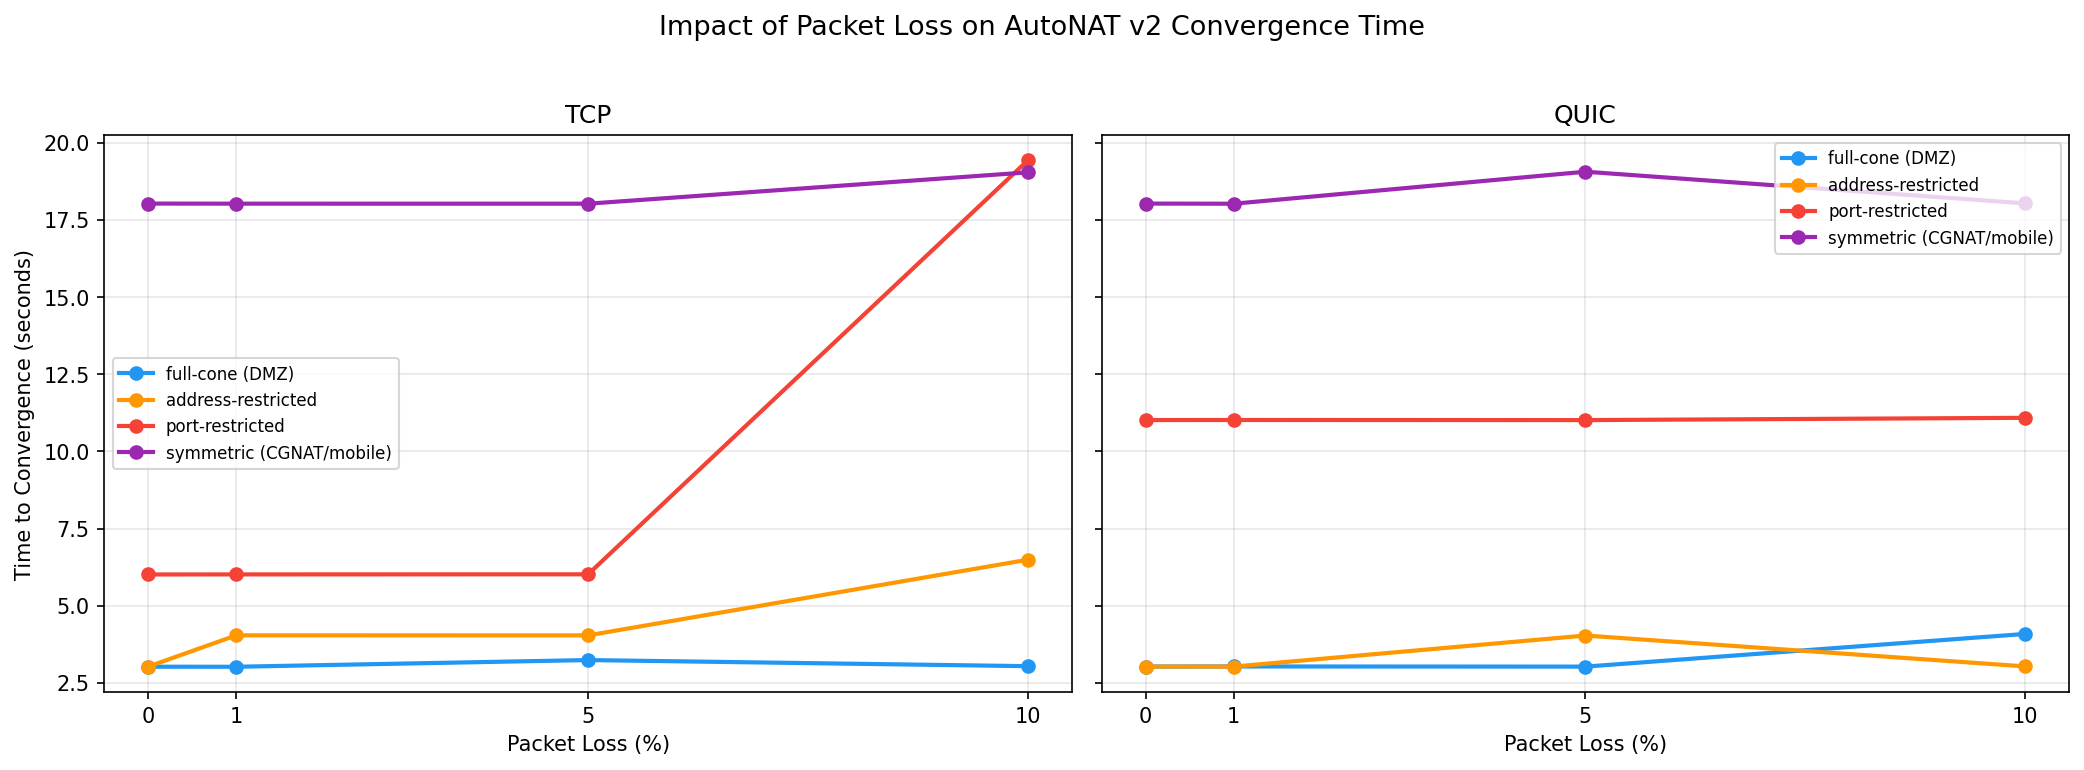
\includegraphics[width=\columnwidth]{04_packet_loss_impact.png}
\caption{Packet loss impact on convergence time. QUIC (right) remains flat; TCP (left) increases steeply at 10\% loss.}
\label{fig:packet-loss}
\end{figure}

%----------------------------------------------------------------------
\section{Results: Protocol Issues}
%----------------------------------------------------------------------

\subsection{Address-Restricted NAT False Positive}

AutoNAT v2's dial-back originates from the server's IP---the same IP the client previously contacted. For ADF NATs, the dial-back succeeds even though arbitrary peers cannot reach the node. We tested 120 runs (60 ADF, 60 APDF control): ADF produces \textbf{100\% FPR}; APDF produces 0\% FPR. The false positive is deterministic---guaranteed by the protocol design. Real-world impact is likely limited as ADF is rare in modern routers~\cite{rfc4787,rfc7857}.

\begin{figure}[htbp]
\centering
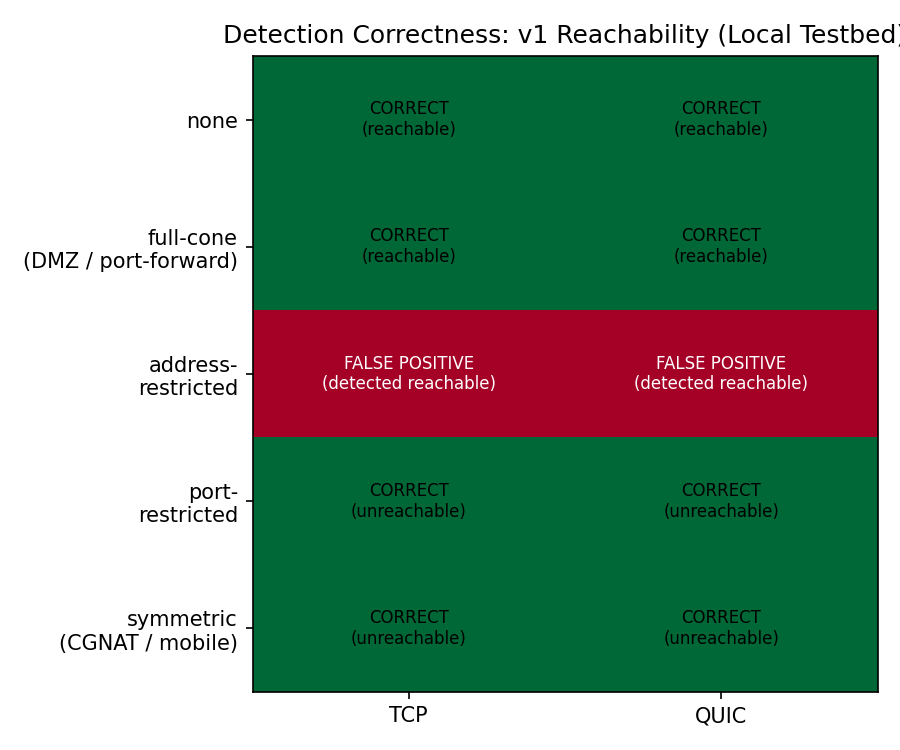
\includegraphics[width=\columnwidth]{05_detection_correctness.png}
\caption{Detection correctness heatmap. Address-restricted NAT is incorrectly classified as reachable (false positive).}
\label{fig:correctness}
\end{figure}

\subsection{Symmetric NAT Silent Failure}

Under symmetric NAT, each connection uses a different external port. No address reaches \texttt{ActivationThresh=4}, so AutoNAT v2 never runs. All symmetric scenarios produce zero events. With \texttt{thresh=1}, symmetric nodes receive an UNREACHABLE determination (correct), showing the silence is threshold-caused and fixable---at the cost of lower address confidence.

\subsection{Threshold Sensitivity}

The activation threshold only affects \emph{observed} address promotion for NATted nodes. No-NAT nodes converge regardless of threshold (their listen address is directly public). This means the threshold is not a hard server-count minimum but an observation-consolidation gate.

%----------------------------------------------------------------------
\section{Results: v1/v2 Integration Gap}
%----------------------------------------------------------------------

\subsection{Independent Signals}

In go-libp2p, v1 emits \texttt{EvtLocalReachabilityChanged} (consumed by DHT, AutoRelay, Address Manager, NAT Service). v2 emits \texttt{EvtHostReachableAddrsChanged} (consumed only by Address Manager). No subsystem except the address manager reads v2 results.

\subsection{v1 Oscillation}

We tested with full-cone NAT (genuinely reachable), 2~reliable + 5~unreliable servers, v1 refresh shortened to 30\,s. Fig.~\ref{fig:gap} shows the representative trace: v2 reaches REACHABLE at 6\,s and stays stable; v1 oscillates PUBLIC$\rightarrow$PRIVATE$\rightarrow$PUBLIC. Across runs: v1 oscillates in \textbf{60\%}; v2 oscillates in \textbf{0\%}.

\begin{figure}[htbp]
\centering
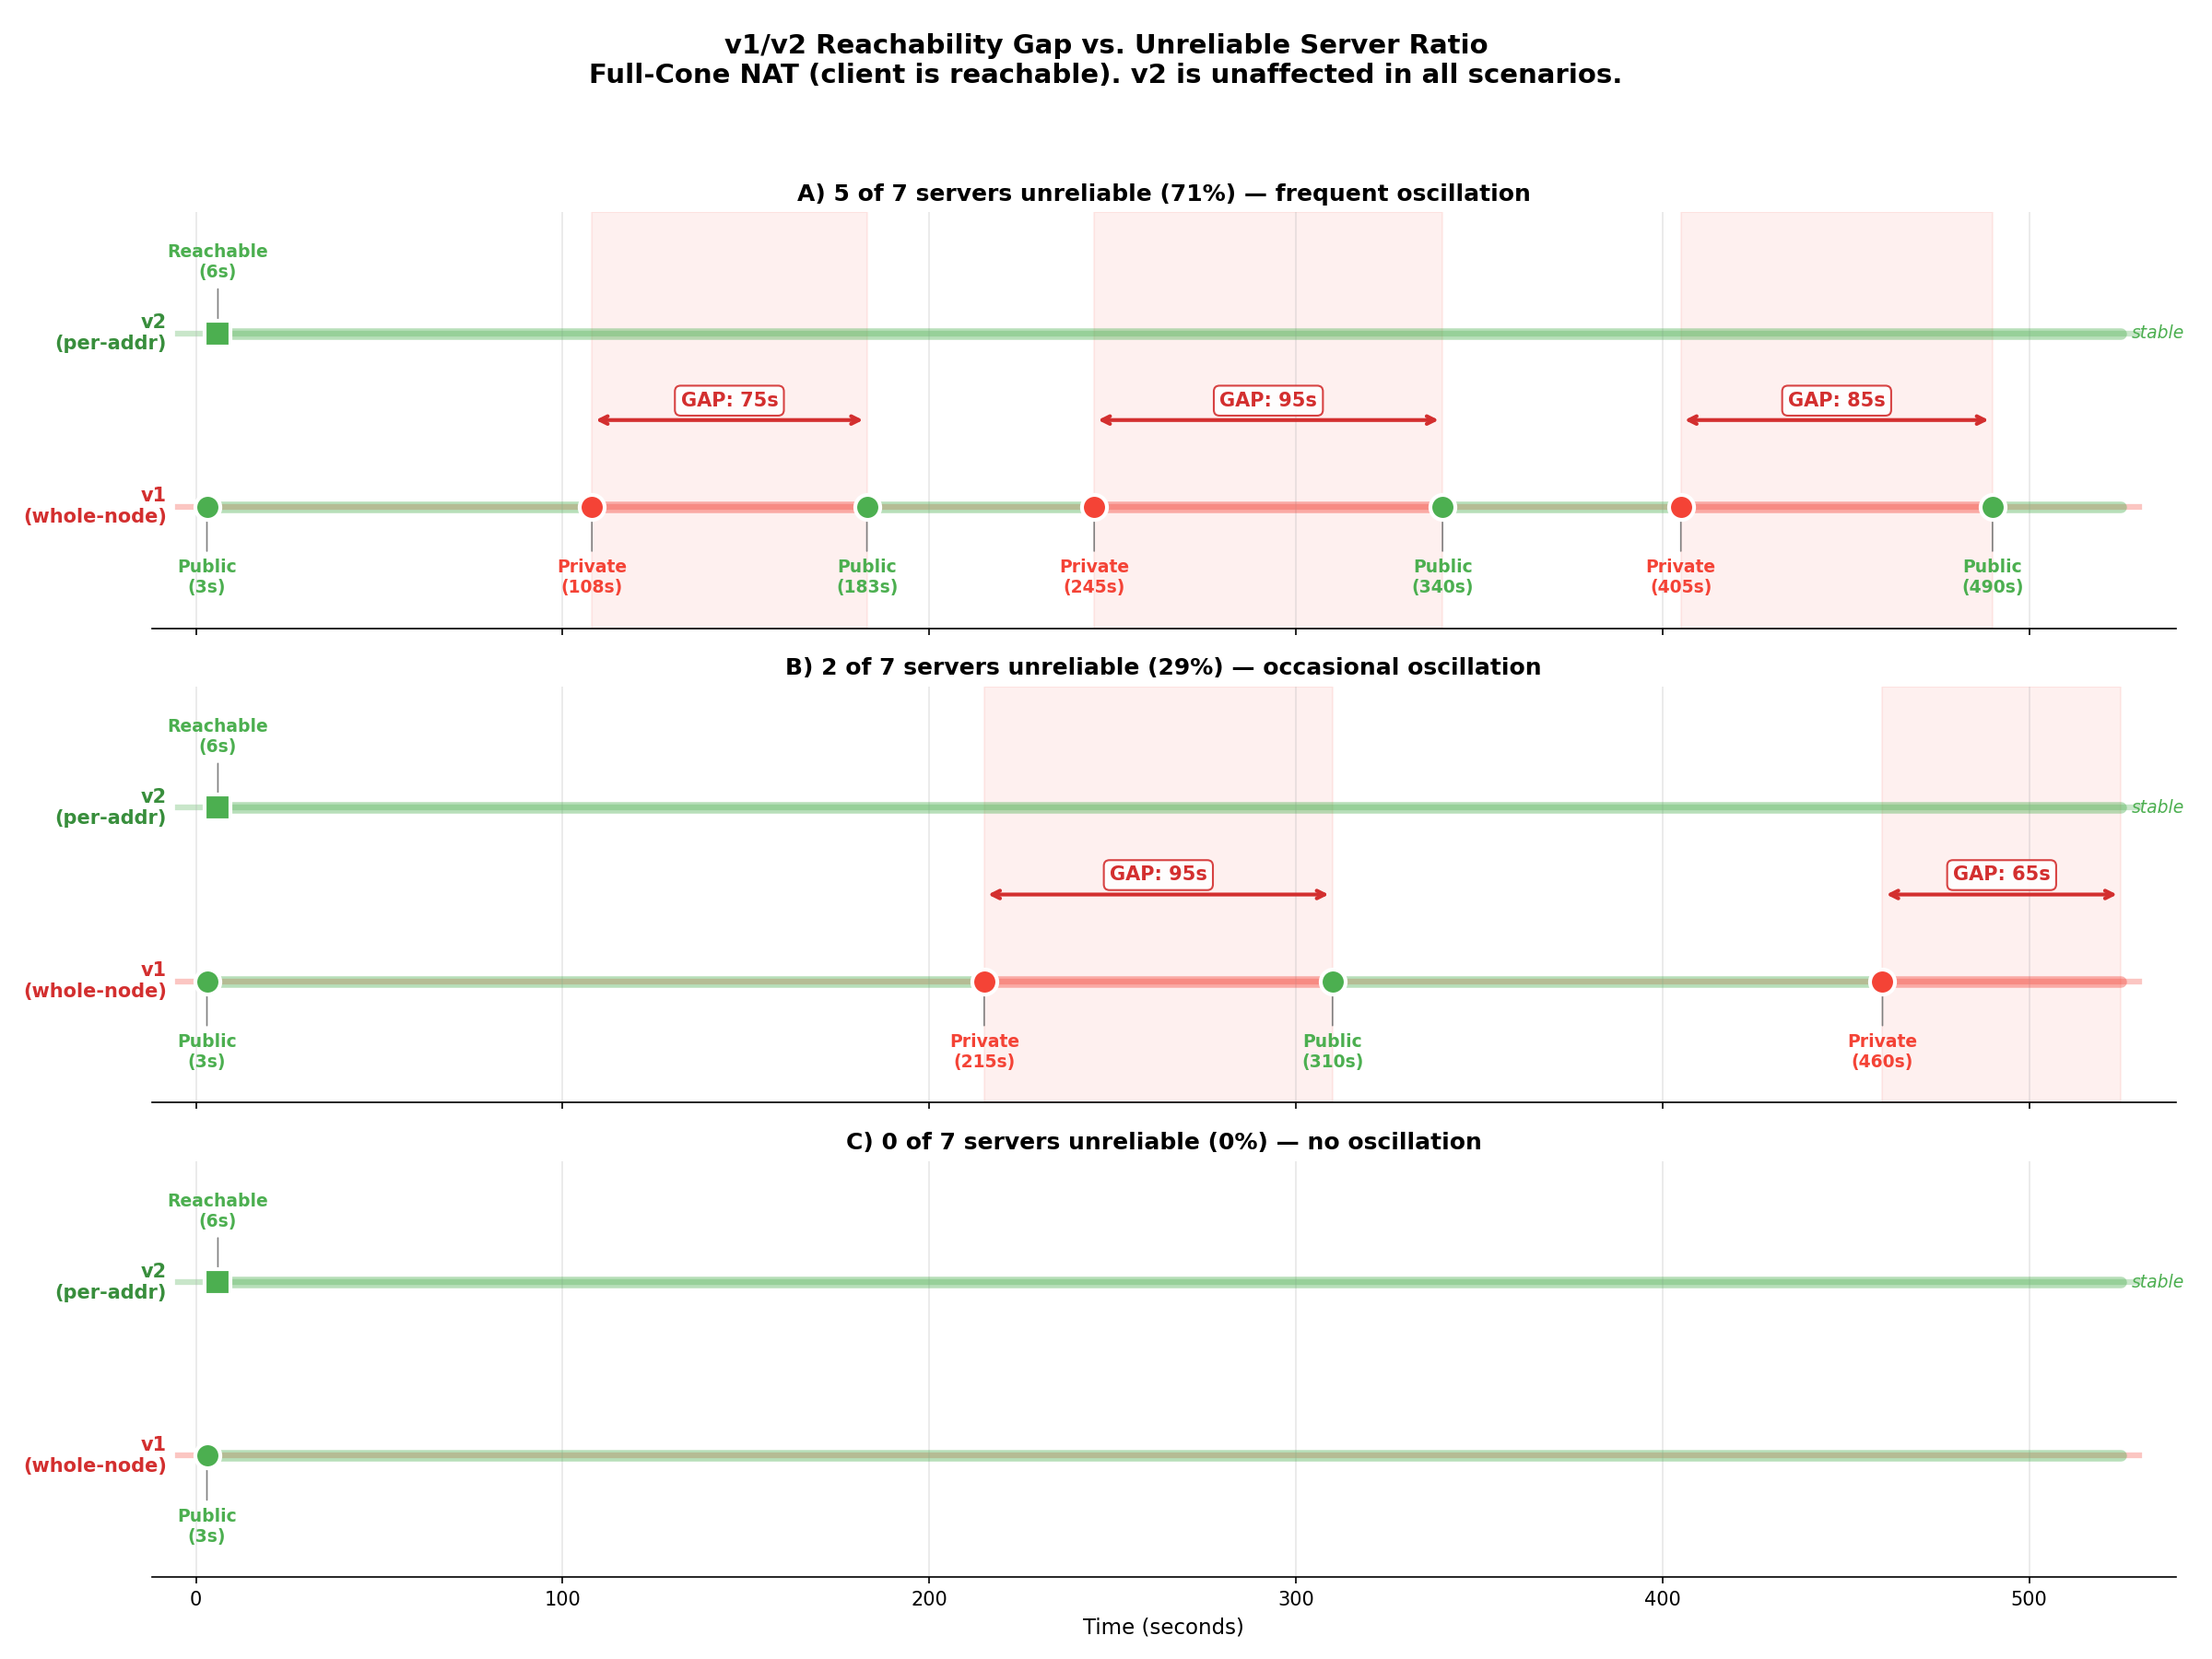
\includegraphics[width=\columnwidth]{10_v1_v2_gap_comparison.png}
\caption{v1/v2 reachability gap. v1 oscillates (red) while v2 stays stable (green) across three unreliable server ratios.}
\label{fig:gap}
\end{figure}

\subsection{DHT Impact}

The Kademlia DHT in \texttt{ModeAuto} subscribes to v1. Each flip triggers server$\leftrightarrow$client mode switching, causing routing table churn. v2's stable results are ignored.

\subsection{Time-to-Update}

Port forwarding toggle detection for port-restricted NAT: 30\,s to detect addition, 69\,s to detect removal. Consistent across transports. Symmetric and address-restricted toggles are not detected (v2 never runs or already false-positive reachable).

%----------------------------------------------------------------------
\section{Results: Cross-Implementation}
%----------------------------------------------------------------------

We tested all three implementations as clients against go-libp2p servers.

\subsection{rust-libp2p: Ephemeral Port Probing}

The rust-libp2p client probes observed connection addresses (ephemeral source ports from Identify) instead of listen addresses. Without go-libp2p's \texttt{ObservedAddrManager} consolidation, every candidate has a unique ephemeral port. Result: \textbf{100\% FNR}. The DHT stays in client mode permanently since no address is ever confirmed. Substrate/Polkadot, rust-libp2p's primary consumer, does not enable autonat.

\subsection{js-libp2p: No Reachability Events}

The \texttt{@libp2p/autonat-v2} package emits no events to consumers. The DHT receives signals indirectly via the address manager. Notably, js-libp2p v1 uses monotonic counters (4 successes / 8 failures) with TTL-based re-evaluation---significantly more oscillation-resistant than go-libp2p v1's sliding window. Helia uses v1 only, not v2.

\subsection{Implementation Comparison}

Table~\ref{tab:cross-impl} summarizes the key differences.

\begin{table}[htbp]
\caption{Cross-Implementation Comparison}
\label{tab:cross-impl}
\centering
\small
\begin{tabular}{@{}llll@{}}
\toprule
Feature & go & rust & js \\
\midrule
Production & Kubo (v1+v2) & None & Helia (v1) \\
Confidence & Window, t=3 & Single probe & Fixed 4/8 \\
Addr filter & ObsAddrMgr & None (bug) & Cuckoo filter \\
Events & Yes & Per-probe & None \\
v2$\rightarrow$DHT & No (v1 only) & Indirect & Indirect \\
v1 osc. resist. & Low & N/A & High \\
\bottomrule
\end{tabular}
\end{table}

\subsection{UDP Black Hole Detector}

go-libp2p's \texttt{UDPBlackHoleSuccessCounter} blocks QUIC dials when too few succeed. The v2 \texttt{dialerHost} shares the main host's counter---on fresh servers, this blocks QUIC dial-backs (false negative). The v1 dialer solved this by disabling the counter (PR~\#2529); v2 should adopt the same approach.

%----------------------------------------------------------------------
\section{Discussion}
%----------------------------------------------------------------------

\subsection{The Protocol Is Sound, the Integration Is Not}

AutoNAT v2 achieves 0\% FNR/FPR in standard scenarios, converges in ${\sim}6$\,s, and never oscillates. The problems lie in integration (v2 results unused by DHT/relay), the address pipeline (observed address activation varies across implementations), and edge cases (ADF false positive, symmetric silence).

\subsection{Recommendations}

\textbf{R1.} Bridge v2 into v1 global flag: ``PUBLIC if any v2-confirmed address is reachable.'' Immediate DHT/relay benefit for Kubo.

\textbf{R2.} Disable black hole detector on \texttt{dialerHost} (matching v1 fix).

\textbf{R3.} Deprecate v1 probing when v2 has data.

\textbf{R4.} rust-libp2p: add observed address consolidation.

\textbf{R5.} js-libp2p: emit reachability events.

\textbf{R6.} Specification: address ADF blind spot via multi-server verification.

\textbf{R7.} Specification: timeout-based inference for symmetric NAT.

\textbf{R8.} Ecosystem: measure real-world NAT type distribution.

\subsection{Limitations}

All experiments run in isolated Docker environments. Real-world conditions include diverse NAT implementations, variable peer counts, and background traffic. We cannot quantify ADF or symmetric NAT prevalence without real-world measurement. Most experiments use single runs; statistical variance is not characterized for latency/loss scenarios. All servers are go-libp2p.

%----------------------------------------------------------------------
\section{Future Work}
%----------------------------------------------------------------------

\subsection{Nebula Queries}

The Nebula DHT crawler~\cite{nebula} stores per-peer protocol lists and agent versions. SQL queries on the existing database can provide AutoNAT v2 adoption rate and transport patterns with no code changes.

\subsection{NAT Classification via ants-watch}

For full NAT type classification, we propose deploying sybil nodes across the DHT keyspace using ants-watch~\cite{ants-watch} on 2--3 VPS with different IPs. Peers connect during normal DHT operations, enabling multi-vantage port comparison: (1)~observed port comparison across vantage points (EIM vs ADPM); (2)~unsolicited dial from uncontacted vantage (EIF vs restricted); (3)~contacted vantage dials from different port (ADF vs APDF). This captures the entire active population, including NATted peers invisible to crawlers.

%----------------------------------------------------------------------
\section{Conclusion}
%----------------------------------------------------------------------

AutoNAT v2 is a substantial protocol improvement: per-address testing, nonce verification, amplification protection, and a robust confidence system that produces 0\% error rates and never oscillates. QUIC transport adds only +1\% convergence time at 10\% packet loss (vs TCP's +147\%).

However, its effectiveness is undermined by integration failures: v1 still controls the DHT and relay in the only production deployment, and v1 oscillates in 60\% of runs with unreliable peers. The two other implementations have critical bugs and no production consumers. The protocol has inherent blind spots for address-restricted NAT (100\% FP) and symmetric NAT (no signal).

The most impactful near-term fix is bridging v2 results into the v1 global flag (R1), immediately benefiting tens of thousands of Kubo nodes. Longer-term, the ecosystem should converge on the per-address model, deprecating the global reachability flag entirely.

%----------------------------------------------------------------------
\balance
\bibliographystyle{IEEEtran}
\begin{thebibliography}{11}

\bibitem{libp2p-specs}
libp2p specifications, \url{https://github.com/libp2p/specs}.

\bibitem{autonat-v1}
AutoNAT v1 protocol, \texttt{/libp2p/autonat/1.0.0}.

\bibitem{autonat-v2-spec}
AutoNAT v2 specification, \url{https://github.com/libp2p/specs/blob/master/autonat/autonat-v2.md}.

\bibitem{rfc4787}
F. Audet and C. Jennings, ``Network Address Translation (NAT) Behavioral Requirements for Unicast UDP,'' RFC~4787, 2007.

\bibitem{trautwein2022}
D. Trautwein, A. Ingen, and D. Vyzovitis, ``Decentralized Hole Punching,'' in \emph{Proc. DINPS}, 2022.

\bibitem{trautwein2025}
D. Trautwein et al., ``Challenging Tribal Knowledge---Large Scale Measurement Campaign on Decentralized NAT Traversal,'' arXiv:2510.27500, 2025.

\bibitem{halkes2011}
G. Halkes and J. Pouwelse, ``UDP NAT and Firewall Puncturing in the Wild,'' in \emph{Proc. PAM}, 2011.

\bibitem{rfc7857}
R. Penno et al., ``Updates to Network Address Translation (NAT) Behavioral Requirements,'' RFC~7857, 2016.

\bibitem{probelab-fork}
probe-lab/go-libp2p fork, branch \texttt{v0.47.0-autonat\_otel}, \url{https://github.com/probe-lab/go-libp2p}.

\bibitem{nebula}
Nebula DHT crawler, \url{https://github.com/probe-lab/nebula}.

\bibitem{ants-watch}
ants-watch DHT sybil framework, \url{https://github.com/probe-lab/ants-watch}.

\end{thebibliography}

\end{document}
